\title{$k$-Means}
\label{chp:k-means}
\author{Harish Tayyar Madabushi}
\institute{The University of Sheffield}
%% \maketitle
%% Add your content here
%% \title{$k$-Means Clustering Algorithm}
\maketitle

The $k$-means clustering algorithm ($k$-means for short) provides a method of finding \emph{structure} in input examples. It is also called the Lloyd--Forgy algorithm as it was independently introduced by both Stuart Lloyd~\cite{lloyd1982least} and Edward Forgy~\cite{Forgy1965ClusterAO}. $k$-means, like other algorithms you will study in this part of the book, is an \emph{unsupervised learning} algorithm and, as such, does not require labels associated with input examples. Recall that unsupervised learning algorithms provide a way of discovering some inherent structure in the input examples. This is in contrast with supervised learning algorithms, which require input examples \emph{and} associated labels so as to fit a hypothesis function that maps input examples to one or more output variables. 

While there are different \emph{structures} that can be extracted from input examples the most intuitive is a \emph{cluster}. Very simply, a cluster is a set of examples that are grouped together, often as a consequence of those examples sharing some similarities. The $k$-means algorithm is one method of finding clusters in input examples. It is important to note that $k$-means requires as input the number of clusters ($k$) and the method of selecting this number is not always obvious. While there are methods of estimating a `good' $k$, some of which we will discuss later in Section \ref{sec:find-k}, this might not always be feasible and, in such instances, one might use algorithms which do not require selecting a value of $k$. You will study some of these other algorithms, such as DBScan, in subsequent chapters of this book. Although clustering provides us with methods of grouping input examples, it does not provide information on the relationship between these resulting groups. For those cases where we might require such relations, one might use algorithms that can extract what is called connectivity information such as  ``Hierarchical Clustering'', yet another unsupervised learning algorithm that is also detailed in subsequent chapters.

This chapter begins by exploring some applications of clustering algorithms, of which $k$-means is by far the most favored because it is simple, intuitive and also effective. The chapter then provides an intuitive overview of the algorithm, before stepping into the details of its implementation including its optimization objective and computational complexity. Finally, we explore some methods of picking $k$, the number of clusters, before then exploring possible extensions of this algorithm. At the end of this chapter you will \begin{enumerate*}[label=(\alph*)]
\item know what $k$-means is and when to use it, 
\item know how to implement $k$-means, and
\item know how to interpret the results. 
\end{enumerate*}

\section{Motivation and Applications}

Why might one want to cluster input examples together and where might such clustering come in handy? Consider the scenario wherein a manufacturer of sweaters is attempting to come up with some fixed sizes. Garment manufacturers must come up with a fixed (and feasible) number of sizes in which to offer their products to ensure that the manufacturing process is tractable. One method of doing this might be to sample the height and weight of potential customers and group them by those who can wear the same size. Notice how, in this example, the height and weight are the input variables and clusters of input examples will provide an estimate of the heights and weights of people who might fit into the same size. 

The applications of extracting structure from data are wide ranging: online retailers, for example, might want to cluster customers into groups who are shown the same offers, computer files that are often required together might be clustered so they can be loaded together, thus reducing load time. Similarly, students might be clustered based on performance so certain groups can be provided additional support.

Clustering is also used to analyze and group DNA sequences extracted from fragments of biological material~\cite{mbs:/content/journal/ijsem/10.1099/00207713-47-4-1145} to allow biologists to both identify species and also find relationships between species' and where a species fits in the overall taxonomy of biological organisms. Notice that in this case, we require methods that additionally provide information regarding the connections between clusters, such as hierarchical-clustering. As such, it is important to choose an algorithm based on the nature of the problem at hand. 

\section{An Intuitive Overview of $k$-means}

Consider a set of input examples each consisting of two input variables as illustrated by Figure \ref{fig:input-data-a}. Be mindful of the fact that both the axes of the figure represent input variables (neither of them are output variables in contrast with supervised learning). The goal is to cluster these examples into $k$ clusters (i.e., $k$ = 3). Take note of the input examples illustrated in the figure below. Think about what the resultant clusters might look like and if 3 is a reasonable value for $k$. 
\begin{figure}
     \centering
     \begin{subfigure}[b]{0.48\textwidth}
         \centering
         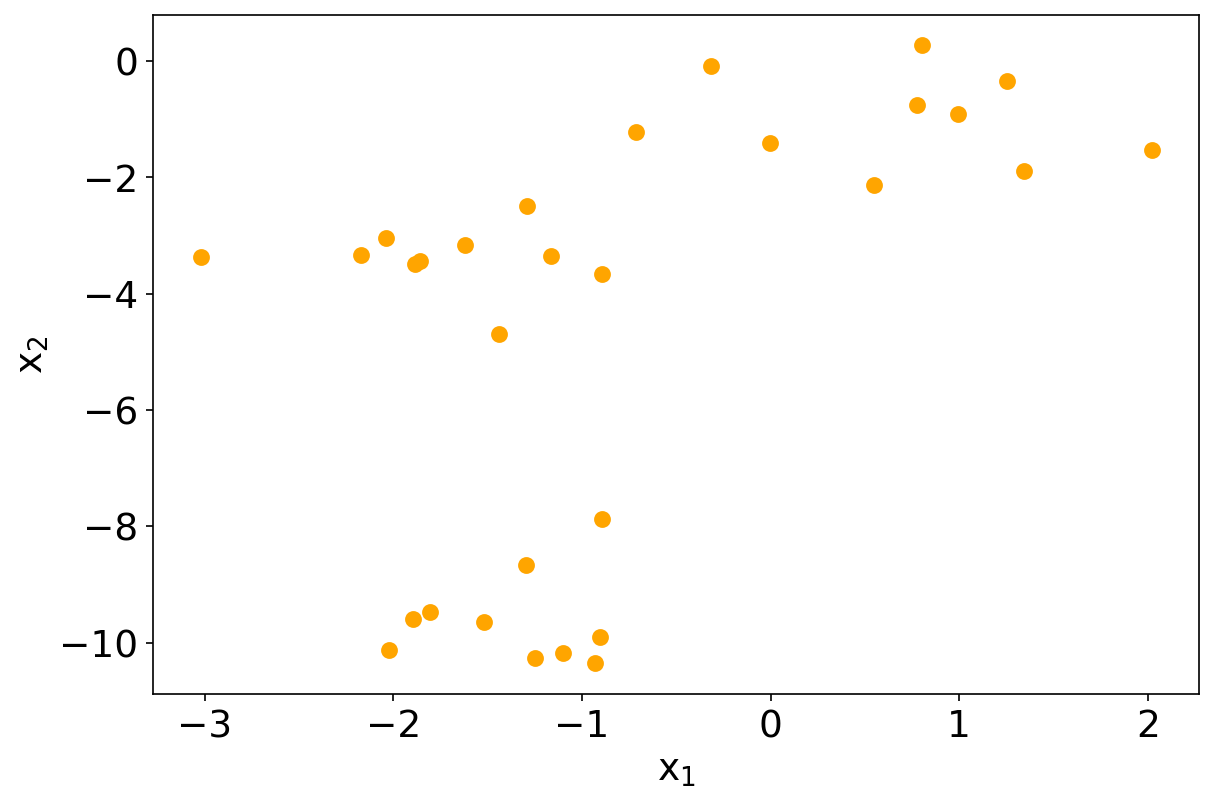
\includegraphics[width=\textwidth]{inputData.png}
         \caption{Input examples}
         \label{fig:input-data-a}
     \end{subfigure}
     \hfill
     \begin{subfigure}[b]{0.48\textwidth}
         \centering
         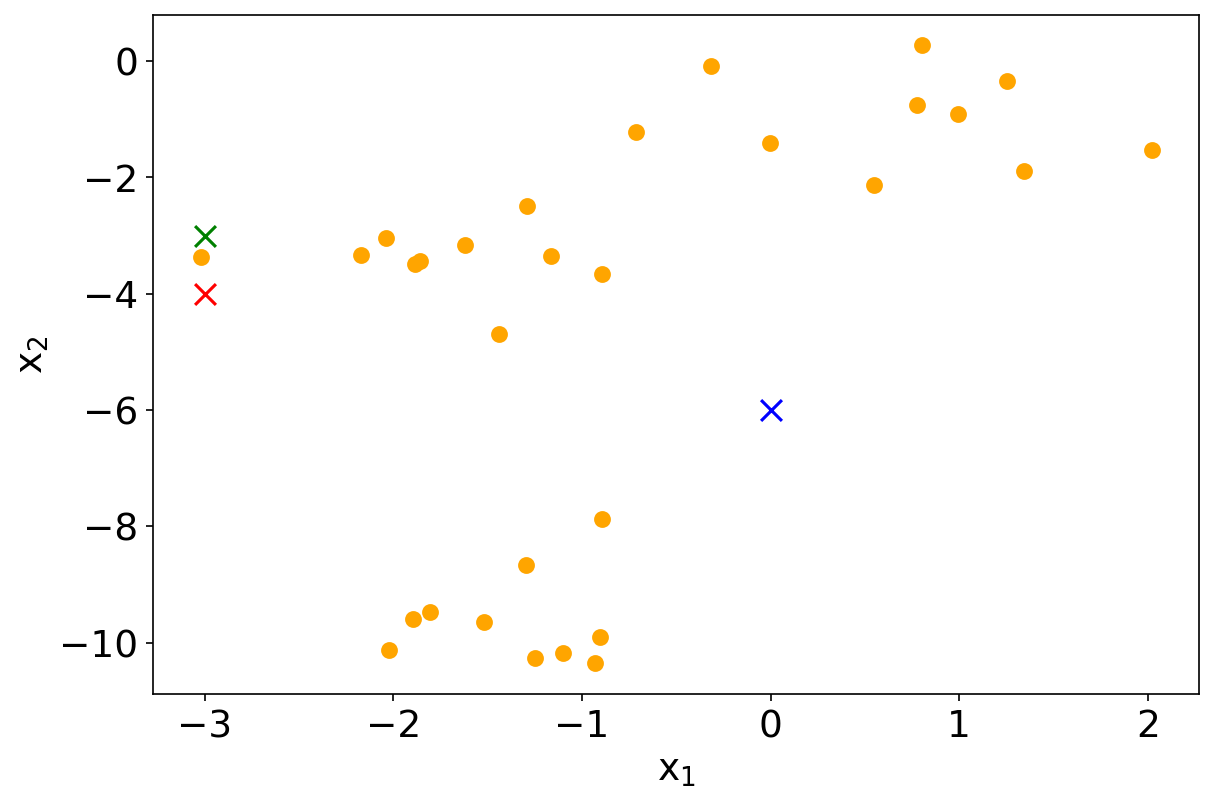
\includegraphics[width=\textwidth]{clusterInit.png}
         \caption{with cluster centroids added.}
         \label{fig:input-data-b}
     \end{subfigure}
     \hfill
        \caption{A visualization of examples in two input variables $x_1$ and $x_2$}
        \label{fig:input-data}
\end{figure}

The $k$-means algorithm takes as input $k$, the number of clusters, and the input examples. It starts by randomly initializing what we call \emph{cluster centroids}, which will eventually be the centroids of our final clusters. Figure \ref{fig:input-data-b} represents a visualization of these centroids alongside the input examples. Notice that each of these randomly initialized centroids has an associated color which we use to represent different clusters. 

$k$-means then performs two steps iteratively: the first is what is called the \emph{cluster assignment} step, wherein each input example is assigned to the cluster centroid that it is ``closest'' to (while we define `close' formally later on, for now, think \emph{close} in two and three dimensions), and the second is the \emph{move centroid} step wherein each cluster centroid is moved to the centroid of the input examples that were assigned to it in step 1. Figure \ref{fig:k-means-loop} illustrates three iterations over these steps. At the end of each iteration the centroid that an example is associated with (its color) can switch based on how the centroids themselves moved. 

Notice how, on the third iteration, there is very little movement of the centroids (Figure \ref{fig:k-means-loop-3-mc}) and how any subsequent iterations will result in no change at all. When this occurs, $k$-means terminates and clusters associated with each cluster centroid are returned. Note that in practice, $k$-means is run for a fixed number of iterations (e.g. 15 -- 20) as the clusters change only minimally after this point (also see Section \ref{sec:complexity}). 

\begin{figure}
     \centering
     \begin{subfigure}[b]{0.48\textwidth}
         \centering
         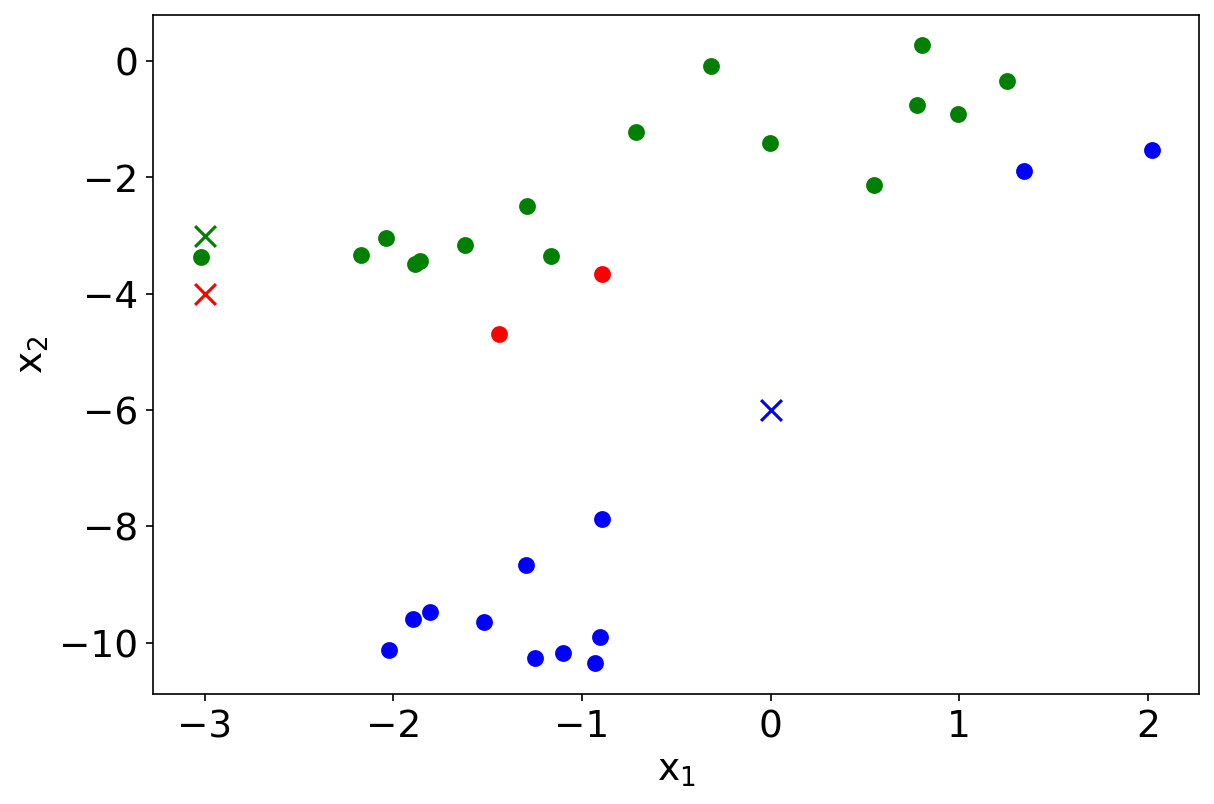
\includegraphics[width=\textwidth]{CA1.png}
         \caption{Iter. 1: Cluster assignment}
         \label{fig:k-means-loop-1-ca}
     \end{subfigure}
     \hfill
     \begin{subfigure}[b]{0.48\textwidth}
         \centering
         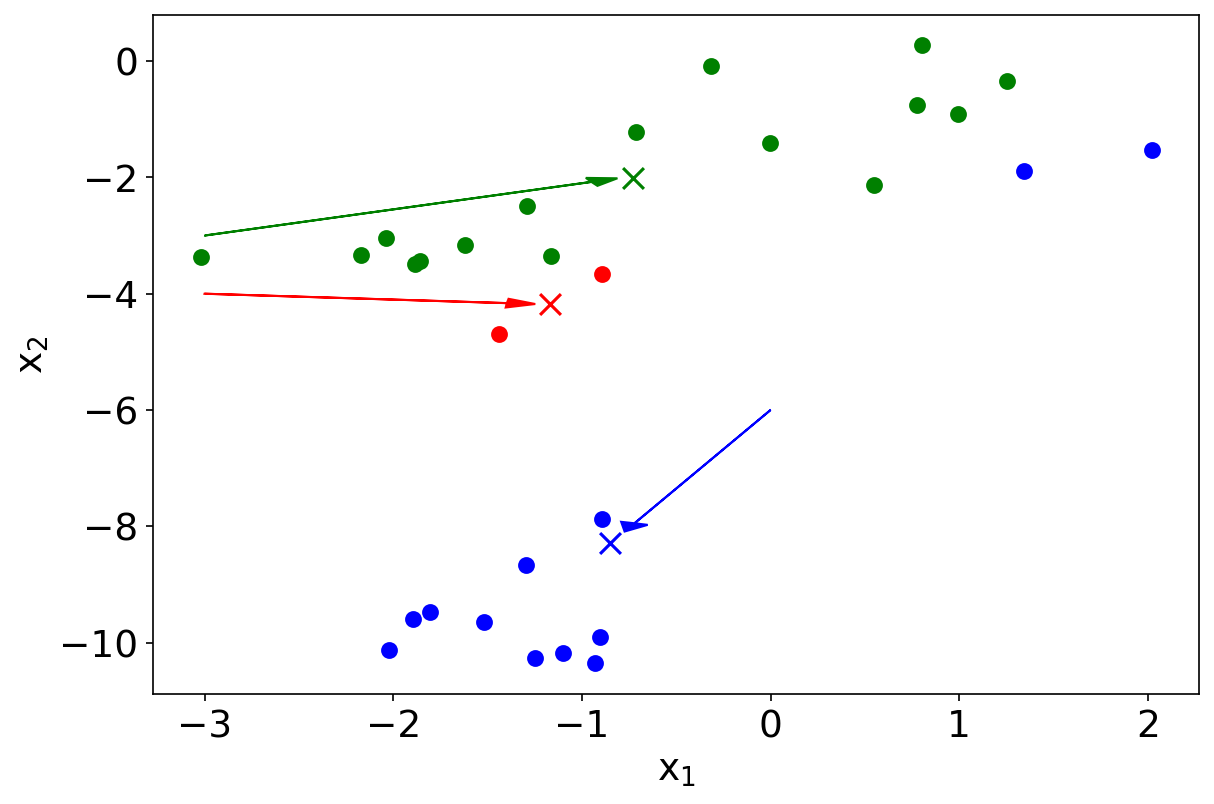
\includegraphics[width=\textwidth]{MC1.png}
         \caption{Iter. 1: Move centroid.}
         \label{fig:k-means-loop-1-mc}
     \end{subfigure}
     \hfill
     \begin{subfigure}[b]{0.48\textwidth}
         \centering
         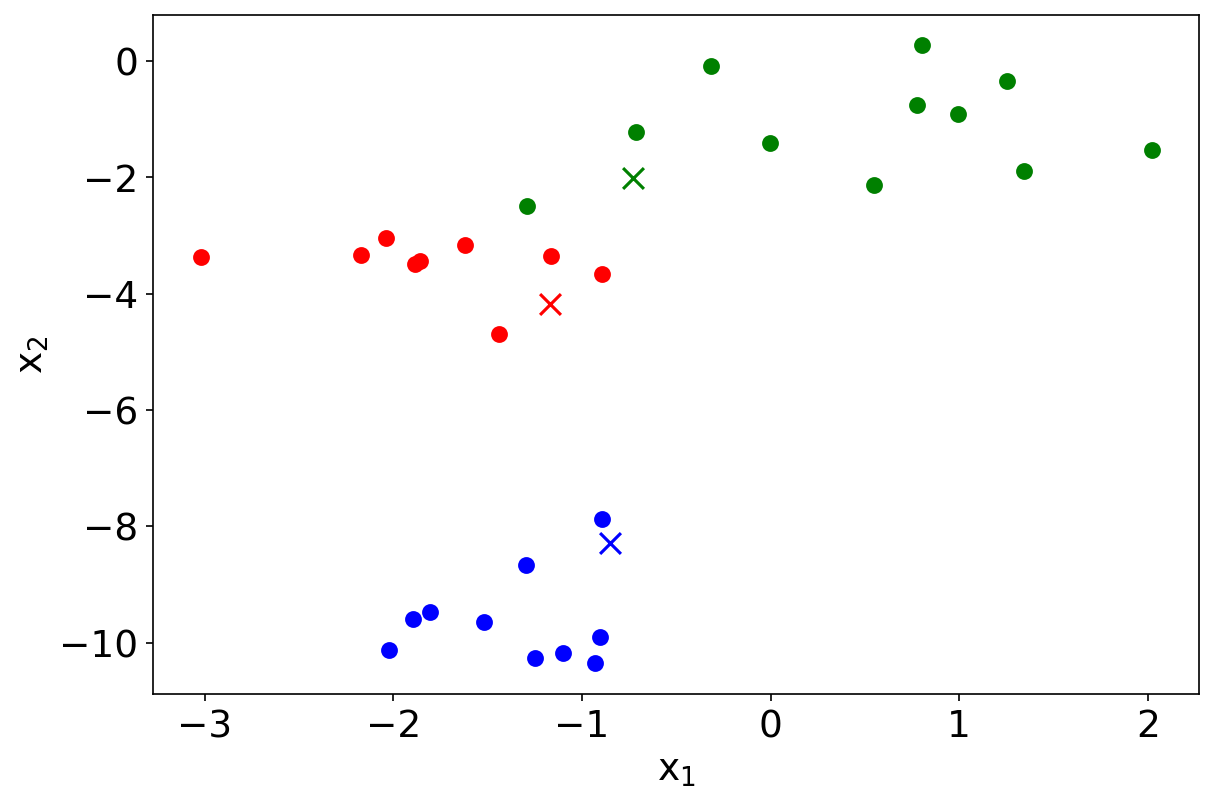
\includegraphics[width=\textwidth]{CA2.png}
         \caption{Iter. 2: Cluster assignment}
         \label{fig:k-means-loop-2-ca}
     \end{subfigure}
     \hfill
     \begin{subfigure}[b]{0.48\textwidth}
         \centering
         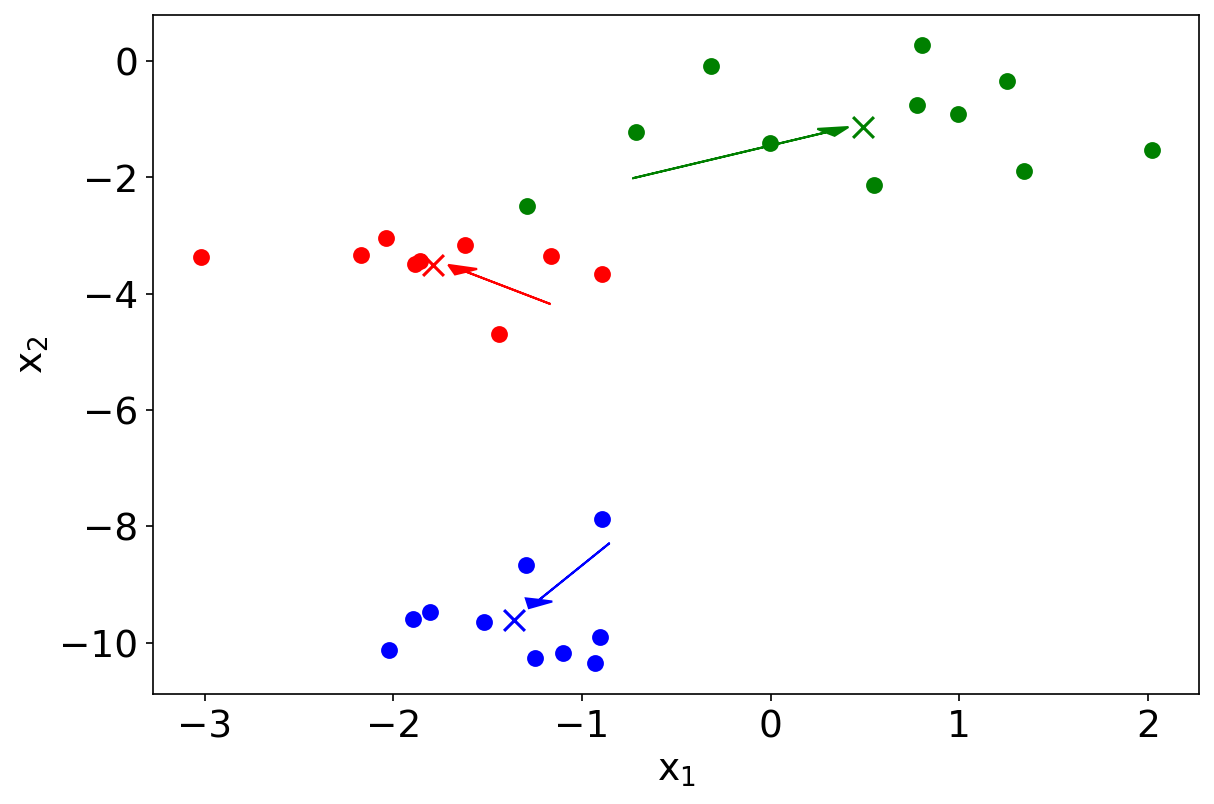
\includegraphics[width=\textwidth]{MC2.png}
         \caption{Iter. 2: Move centroid.}
         \label{fig:k-means-loop-2-mc}
     \end{subfigure}
     \hfill
     \begin{subfigure}[b]{0.48\textwidth}
         \centering
         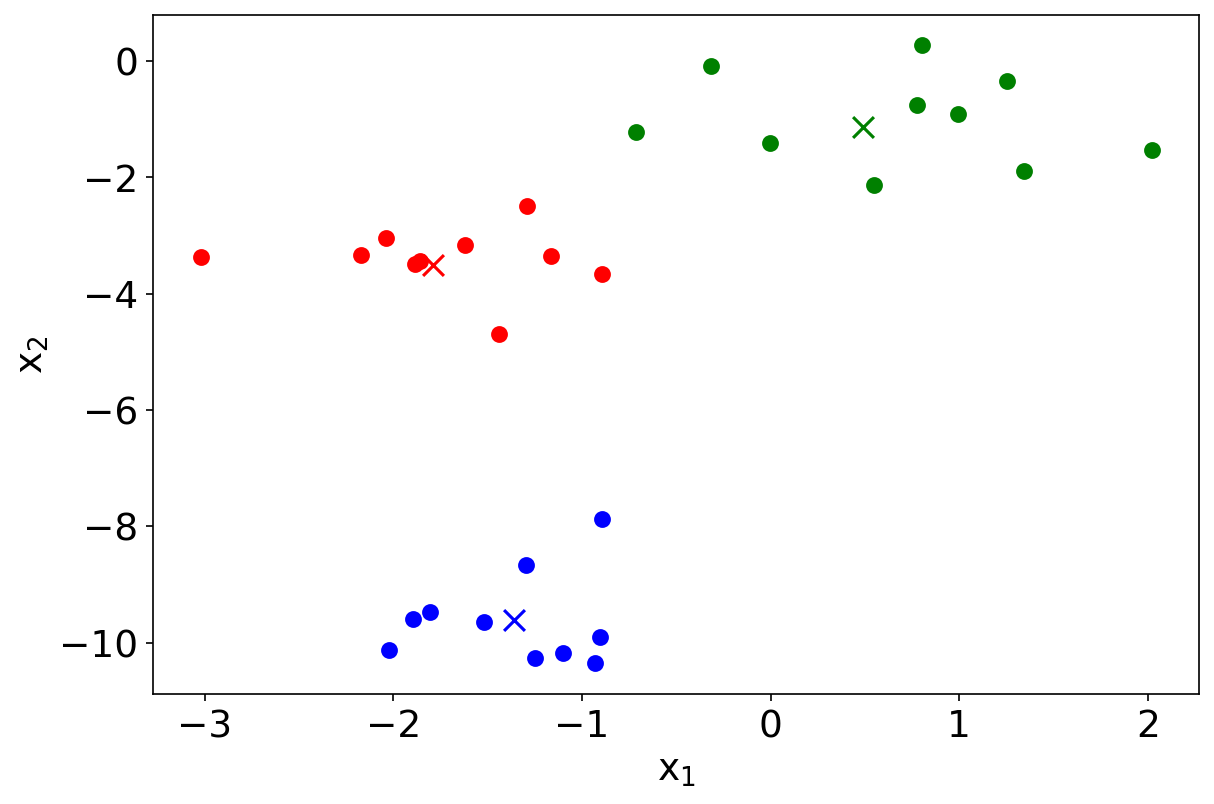
\includegraphics[width=\textwidth]{CA3.png}
         \caption{Iter. 3: Cluster assignment.}
         \label{fig:k-means-loop-3-ca}
     \end{subfigure}
     \hfill
     \begin{subfigure}[b]{0.48\textwidth}
         \centering
         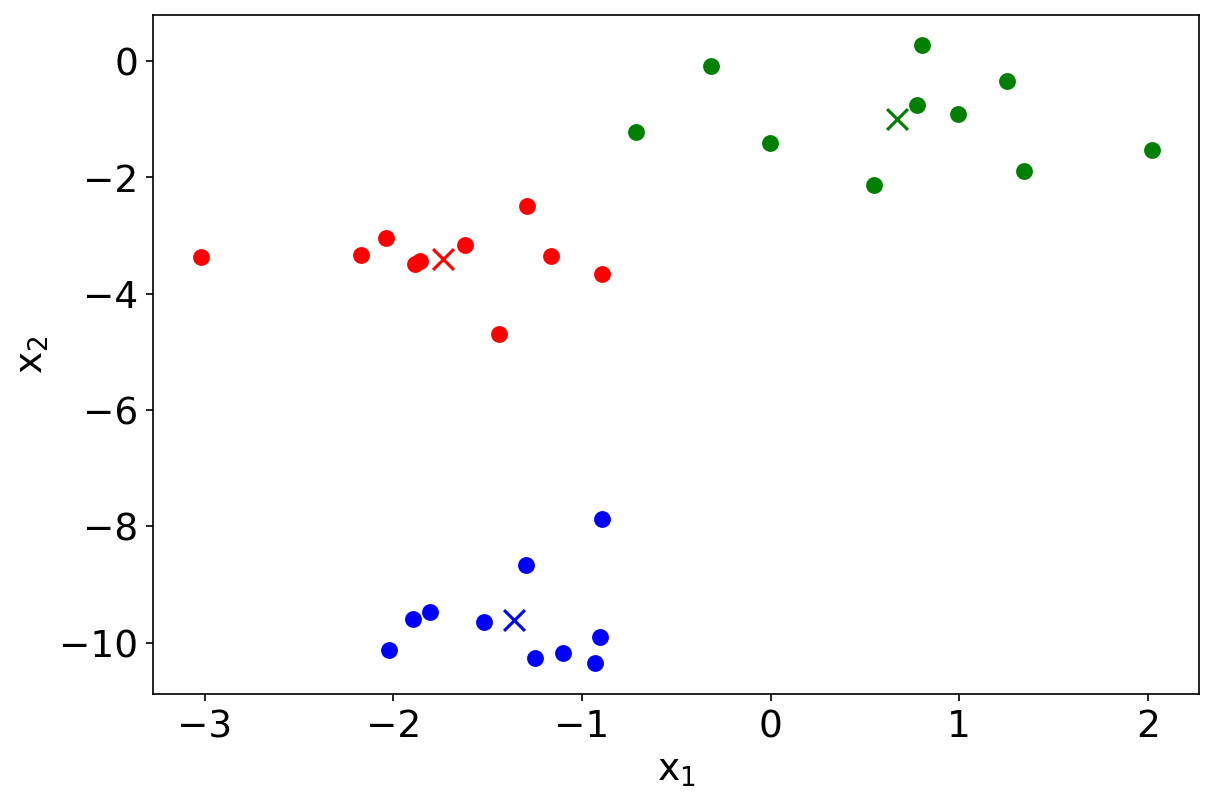
\includegraphics[width=\textwidth]{MC3.png}
         \caption{Iter. 3: Move centroid.}
         \label{fig:k-means-loop-3-mc}
     \end{subfigure}
        \caption{A visualization of $k$-means performing \emph{cluster assignment} and \emph{move centroid} over 3 iterations. Notice the negligible movement of centroids in iteration 3.}
        \label{fig:k-means-loop}
\end{figure}

It is important to remember that $k$-means is sensitive to both the initialization of the cluster centroids~\cite{CELEBI2013200} and the value of $k$. What this implies is that the output clusters will change (sometimes dramatically) based on either of these. So far, we've gained a high level understanding of $k$-means. In the next section, we will formalize this intuition and, additionally, discuss the \emph{optimization objective} for $k$-means, which provides a way of evaluating each of the different cluster assignments associated with different initializations and values of $k$. As a result, we can pick the ``best'' cluster assignment from amongst several different ones. 

\section{$k$-means: The internals}

Now that we have an intuitive overview of the $k$-means algorithm, let us explore the algorithm more formally. To begin with, let us revisit the terminology we will be using: The $n$ input examples are denoted as $\mathcal{T} = \{ \mathbf{x}^{(1)}, \mathbf{x}^{(2)}, ... \mathbf{x}^{(n)}\} $ each consisting of $m$ input variables (each person's details in the sweater example above consists of height and weight which are the input variables), and $\{ \boldsymbol{\mu}_1, \boldsymbol{\mu}_2, ... \boldsymbol{\mu}_k\}$ denote the $k$ cluster centroids.  $\{\mathcal{C}^{(1)}, \mathcal{C}^{(2)}, ..., \mathcal{C}^{(k)}\}$ denote the \emph{sets} consisting of the indexes of input examples assigned to the corresponding cluster centroid. Specifically, $\mathcal{C}^{(1)}$ is a set that contains the indexes of input examples assigned to the cluster centroid $\boldsymbol{\mu}_1$ and so on -- for example, $\mathcal{C}^{(1)}$ might be $\{ 1, 4\}$, which would imply that the input examples $\mathbf{x}^{(1)}$ and $\mathbf{x}^{(4)}$ are assigned to the cluster centroid $\boldsymbol{\mu}_1$. 

%%%%%%%%%%%%%%%%%%%%%%%% ALGORITHM
\begin{algorithm}[ht!]
	%\renewcommand{\baselinestretch}{0.8}
	\caption{k-means algorithm}
    
    Parameters: Input examples {$\mathbf{x}^{(1)}$, $\mathbf{x}^{(2)}$, \dots, $\mathbf{x}^{(n)}$ } and the number of clusters, $k$.
    
    Output: $k$ clusters ($\{\mathcal{C}^{(1)}, \mathcal{C}^{(2)}, ..., \mathcal{C}^{(k)}\}$).
    
	\begin{algorithmic}[1] 
		\STATE{Initialize (randomly) $k$ cluster centroids $\{ \boldsymbol{\mu}_1, \boldsymbol{\mu}_2, ... \boldsymbol{\mu}_k\} \in \mathbb{R}^m$}
		
        \REPEAT
		\FOR{$i = 1$ to $k$}
		\STATE{ $\mathcal{C}^{(i)} := \text{indexes of input examples whose ``closest'' cluster centroid is } \boldsymbol{\mu}_i$} %\COMMENT{``Cluster Assignment''}
		\ENDFOR
        \FOR{$i = 1$ to $k$}
        \STATE{ $\boldsymbol{\mu}_i := \text{center of input examples assigned to }\mathcal{C}^{(i)}$}  %\COMMENT{``Move Centroid''}
        \ENDFOR

		\UNTIL No change to clusters ($\{\mathcal{C}^{(1)}, \mathcal{C}^{(2)}, ..., \mathcal{C}^{(k)}\}$) between iterations. 
		
	\end{algorithmic}
	\label{algo:k-means}
\end{algorithm}
%%%%%%%%%%%%%%%%%%%%%%%% ALGORITHM

Consider the $k$-means clustering algorithm presented above (Algorithm \ref{algo:k-means}). The algorithm takes as input the number of required clusters $k$ and the input examples ({$\mathbf{x}^{(1)}$, $\mathbf{x}^{(2)}$, \dots, $\mathbf{x}^{(n)}$ }), and returns the $k$ clusters ($\{\mathcal{C}^{(1)}, \mathcal{C}^{(2)}, ..., \mathcal{C}^{(k)}\}$) consisting of indexes associated with input examples. Notice that the first \emph{for} loop (lines 3 -- 5) performs cluster assignment and second (lines 6 -- 8) performs the move centroid step. It should be noted that some implementations of $k$-means use an array of length $n$ to keep track of the index of the closest centroid to each input example instead of, as we have done, $k$ sets to keep track of the indexes of input examples closest to each centroid. Note that these are equivalent. 

The cluster assignment step requires us to find input examples that are closer to a given cluster centroid than any of the other cluster centroids. We do this by finding the \emph{Euclidean distance} between each input example and all of the cluster centroids and picking the one that is closest. The combination of cluster assignment and move centroid allow $k$-means to generate clusters with minimal \emph{within-cluster variance}. It is possible to use other distance measures (e.g. cosine, cityblock or squared Euclidean distance) in place of Euclidean distances and some implementations of $k$-means 
do provide these options. However, these other measures do not result in clusters with minimal within-cluster variance and the reasoning for convergence of the algorithm that we provide in Section \ref{sec:converge} relies on the use of Euclidean distance. As such, these other measures might result in the algorithm not converging.
In the next section, we will discuss the optimization objective associated with $k$-means and use it to understand how the two steps of the algorithm translate to minimizing within-cluster variance. 

\subsection{Optimization Objective}
\label{section:optimization-objective}

Let's define $\mu(\mathbf{x}^{(i)})$ to represent the cluster centroid that input example $\mathbf{x}^{(i)}$ is assigned to. Recall that $\mathcal{C}^{(i)}$ is a set that contains the indexes of input examples assigned to the cluster centroid $\boldsymbol{\mu}_i$. Therefore, $\mu(\mathbf{x}^{(i)})$ can be written as $\mu(\mathbf{x}^{(i)}) = \boldsymbol{\mu}_j \iff i \in \mathcal{C}^{(j)}$, which expresses the fact that $\mu(\mathbf{x}^{(i)})$ will be equal to $\boldsymbol{\mu}_j$ (a given cluster centroid $j$) \emph{if and only if} $i$ is an element of $\mathcal{C}^{(j)}$. Notice that $i$ being an element of $\mathcal{C}^{(j)}$ would in turn imply that the input example $\mathbf{x}^{(i)}$ is assigned to $\boldsymbol{\mu}_j$. 

Notice that if a centroid is a \emph{good} representation of a set of input examples in a cluster, then it would be ``close'' to each of them. As such, a good measure of this is the sum of the squared distance between the cluster centroid of a cluster and each of the constituent input examples associated with that cluster. This measure is called the \emph{residual sum of squares} (RSS) and is expressed with respect to the cluster centroids ($\{ \boldsymbol{\mu}_1, \boldsymbol{\mu}_2, ... \boldsymbol{\mu}_k\}$) and the cluster assignments ($\{\mathcal{C}^{(1)}, \mathcal{C}^{(2)}, ..., \mathcal{C}^{(k)}\}$) by Equation \ref{eq:rss} below.

\begin{equation}
    RSS(\mathcal{C}^{(1)}, \mathcal{C}^{(2)}, ..., \mathcal{C}^{(k)}, \boldsymbol{\mu}_1, \boldsymbol{\mu}_2, ..., \boldsymbol{\mu}_k) = \mathlarger{\mathlarger{\sum}}_{i = 1}^{n} \norm{ \mathbf{x}^{(i)} - \mu(\mathbf{x}^{(i)}) }^2
    \label{eq:rss}
\end{equation}

Since the RSS represents how well our cluster assignment is doing, we can use it to build an \emph{optimization objective} where we aim to minimize the RSS with respect to the centroids and the cluster assignments. We normalize the RSS by the number of input examples so as to make this value comparable across different sets of inputs. The resultant optimization objective is given by Equation \ref{eq:argmin}.

\begin{equation}
    \underset{\rm \substack{ \mathcal{C}^{(1)}, \mathcal{C}^{(2)}, ..., \mathcal{C}^{(k)} \\ \boldsymbol{\mu}_1, \boldsymbol{\mu}_2, ..., \boldsymbol{\mu}_k }}{\rm \text{min}}~~\frac{1}{n} RSS(\mathcal{C}^{(1)}, \mathcal{C}^{(2)}, ..., \mathcal{C}^{(k)}, \boldsymbol{\mu}_1, \boldsymbol{\mu}_2, ..., \boldsymbol{\mu}_k)
    \label{eq:argmin}
\end{equation}

In fact, the $k$-means algorithm presented in Algorithm \ref{algo:k-means} does exactly what is required by Equation \ref{eq:argmin}, that is, it minimizes the RSS. This is because the first step -- the cluster assignment step -- minimizes the RSS with respect to the cluster assignment ($\mathcal{C}^{(1)}, \mathcal{C}^{(2)}, ..., \mathcal{C}^{(k)}$), while holding the cluster centroids constant, and the second step -- the move centroid step -- minimizes the RSS with respect to the centroids ($\boldsymbol{\mu}_1, \boldsymbol{\mu}_2, ..., \boldsymbol{\mu}_k$), while holding the cluster assignment constant. Also, notice that, for a given cluster, the right hand side of Equation \ref{eq:rss} is the within-cluster variance that $k$-means is implicitly minimizing.  

\subsection{Time Complexity}
\label{sec:complexity}
Let us now consider the time complexity of the $k$-means algorithm. The algorithm relies heavily on computing vector distances and adding vectors (to calculate the centroids), both of which have a time complexity of $\mathcal{O}(m)$, where $m$ is the number of input variables. The cluster assignment step requires the calculation of distances between $k$ centroids and $n$ input examples, and so has an overall complexity of $\mathcal{O}(mkn)$. The move centroid step requires that we perform a total of $n$ additions (across different clusters), each a vector of length $m$ resulting in a complexity of $\mathcal{O}(nm)$. Therefore, the complexity of each iteration is $\mathcal{O}(mkn)$ and the overall complexity of the algorithm over $i$ iterations is $\mathcal{O}(mkni)$. 

Notice that the time complexity we've defined is reliant of the number of iterations $i$, which is relatively difficult to calculate. In the worst case, the complexity of $k$-means, when run until convergence, is superpolynomial~\cite{10.1145/1137856.1137880}. However, in practice, cluster assignments change very little after a relatively small number of iterations and so $k$-means is usually run for a fixed number of iterations~\cite[Chapter~16]{manning2008introduction}.

\subsection{Convergence}
\label{sec:converge}
Does $k$-means always reach a ``stable'' state wherein further iterations do not lead to changes to either the cluster centroids or the cluster assignments? Is it possible that the cluster centroids continue to move around indefinitely, thus leading to a scenario wherein $k$-means does not terminate? It turns out that this is not the case and that $k$-means does always converge (as long as we use Euclidean distance). We can show that $k$-means converges by showing that the RSS monotonically decreases (or remains the same) as a result of the combination of cluster assignment and move centroid. Remember that, in practice, $k$-means is not run until convergence, but for a fixed number of iterations (see also Section \ref{section:optimization-objective}). 

Observe that if the cluster assignment step changes the centroid that an input example is assigned to, then the distance between the input example and that new centroid it is now assigned to (which contributes to the RSS) will necessarily decrease. If the new distance was going to be larger, the cluster assignment step would not have performed this assignment. With regard to the move centroid step, intuitively, it should be clear that the point from which the sum of the distance to all points in a cluster is minimal is its center and so such a move will never increase the RSS. For a  more formal analysis, see ~\cite[Chapter~16]{manning2008introduction}.

Given the monotonic decrease of the RSS and the fact that there are only a finite number of possible clusterings, $k$-means is guaranteed to converge to a \emph{local minimum} and terminate \emph{as long as input examples that are equidistant from multiple cluster centroids are allocated to one in a consistent manner}. This is important as not doing so could result in $k$-means not terminating as such examples oscillate between centroids. Now that we have established that $k$-means does in fact terminate and that it does so at some local minimum, the next section discusses methods of attempting to find the solution that is globally optimal (or as close to it as is practical).

\section{Random Initialization}

As mentioned earlier, $k$-means is highly sensitive to random initialization of the cluster centroids -- different initialization can result in very different clusters. Each clustering represents one possible local minimum of the RSS as described in Section \ref{section:optimization-objective} above. Finding a globally optimal solution requires running the algorithm multiple times using different random initialization and picking the one with the least RSS. Notice that this method is not guaranteed to provide a global optimum -- it only increases the likelihood of finding one, and this likelihood continues to increase as the number of attempts increases. In practice, $k$-means, like most machine learning algorithms, is run 10 times, and we pick the clustering with the least RSS. 

There are methods of randomly initializing the centroids that can sometimes speed up convergence. One such method is to randomly partition the input examples into $k$ sets and to use the centroids of these sets as initial cluster centroids. Another method is to similarly partition \emph{some} input examples into $k$ sets each containing a relatively small number of examples (e.g. 10) and then use their centroids as the initial cluster centroids. For more initialization methods and a formal analysis of their characteristics, see~\cite{CELEBI2013200,10.5555/645527.657466}. 

\section{Optimal Number of Clusters}
\label{sec:find-k}
Given that the $k$-means algorithm requires the number of clusters as input, we must be able to (roughly) determine this number independently. Notice that we cannot rely solely on ``minimizing RSS'' as we did when selecting the best initialization. This is because the value of the RSS will reduce with the increase in the value of $k$ (up to some point). Therefore, the standard method of establishing the optimal number of clusters is by using the \emph{Elbow Method}. This requires one to plot the RSS against a varying number of clusters as in Figure \ref{fig:elbow} and to pick a $k$ at a point where the curve bends the most (the \emph{elbow}), as highlighted in the plot. Notice that this allows us to pick a $k$ beyond which the `gains' obtained by adding a cluster are not worth the `cost'. Importantly, for each $k$, the $k$-means algorithm must be run multiple times (about 10) using different initialization and the best clustering for that $k$ is chosen to be the run with the minimal RSS. 

\begin{figure}
    \centering
    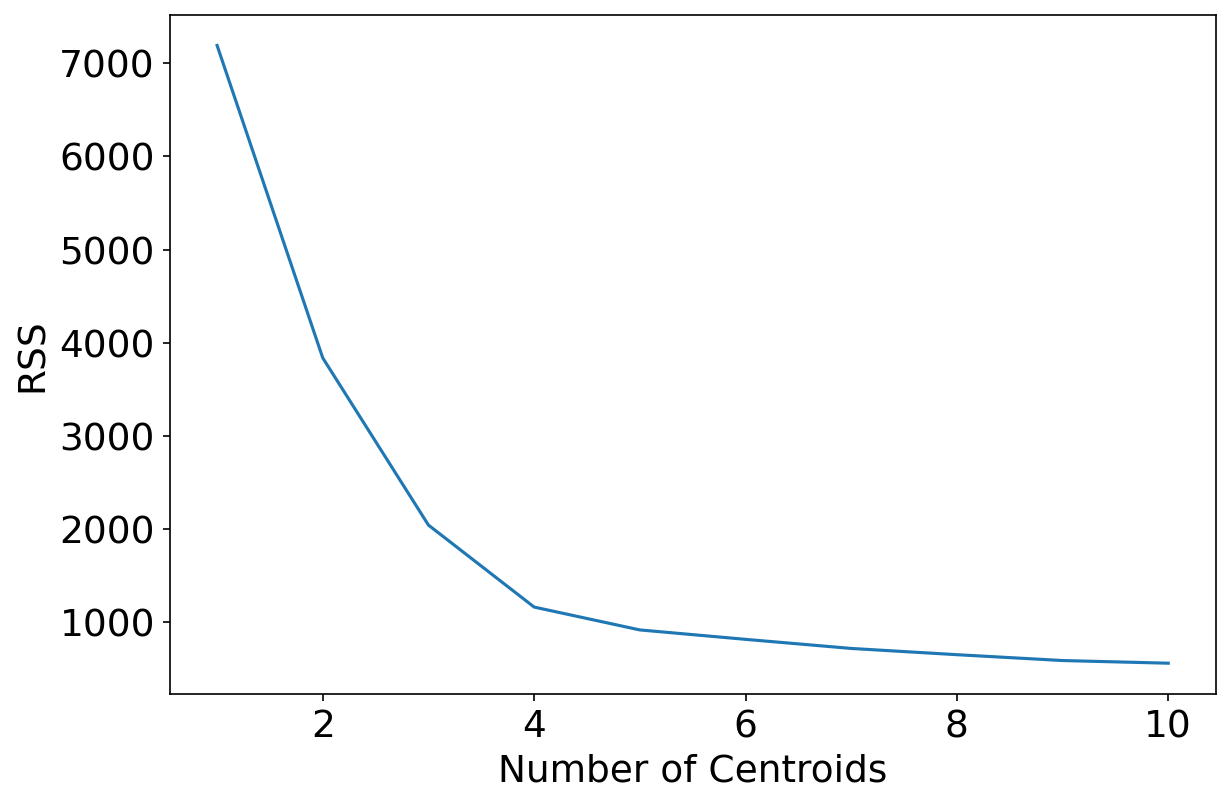
\includegraphics[width=0.7\textwidth]{Elbow.png}
         \caption{Plot of how RSS varies with change in the number of cluster centroids. Notice how $k = 4$ provides an ``Elbow''.}
         \label{fig:elbow}
\end{figure}
     

The other way of establishing the number of clusters is based on what these clusters are going to be used for in a downstream task. For example, if we are clustering customers (by a combination of their heights and weights) so as to come up with a fixed number of sweater sizes (e.g. XS, S, M, L, XL), then we could use the number of sizes we intend to create (in this case 5) as our $k$. 

\subsection{Empty assignments}

As the number of clusters increases, the cluster assignment step of $k$-means might result in one or more cluster centroids being assigned no input examples. As a result, the move centroid step will lead to errors because the centroid of zero input examples does not exist. There are a couple of ways to handle this: a) to ignore such centroids in all future steps of $k$-means, thus resulting in less than $k$ clusters or, b) keeping such centroids in their prior positions and continuing with the algorithm. What you choose to do will depend on the requirements of your problem, but not handling this case will result in your algorithm failing. 

\section{Summary and Discussion}

In this chapter, we discussed the need for methods of discovering both standalone and connected clusters in input examples. Given this motivation, we studied the $k$-means algorithm, which is only one, albeit the most popular algorithm for finding clusters amongst input examples. We discussed the algorithm both intuitively and more formally with a particular emphasis on those aspects of the algorithm that are important to be aware of so as to effectively implement and use $k$-means. Remember that $k$-means requires the definition of $k$, which is its biggest handicap. Additionally, notice that $k$-means can only capture clusters that are \emph{hyperspherical} (i.e. circle in two dimensions, sphere in three, \dots) and so might not always be appropriate in certain situations. However, $k$-means is an intuitive algorithm, which, when run for a fixed number of iterations as is generally the practice, is also efficient. 

\section{Exercises}

\paragraph{Exercise 1} 
The $k$-means algorithm is run with $k$ set to 2. During a particular iteration, the cluster centroids of the two clusters are A: $(15, 3)$ and B: $(12, 18)$. Which of the two centroids will the following input examples be assigned to and why: $(1, 2)$ and $(8, 9)$ 

\paragraph{Exercise 2}
Assume that a special chip, designed to optimize vector manipulation, is able to calculate the distance between vectors and to add vectors in constant time. What would the time complexity of the $k$-means algorithm be, assuming we always run it for a fixed number of iterations (say 15)?

\paragraph{Exercise 3} 
Implement the $k$-means algorithm and additionally ensure that, for a given input, your implementation: 
    \begin{enumerate}
        \item Executes $k$-means for a varying number of clusters (e.g. between 2 and 10).
        \item Executes $k$-means multiple times (e.g. 10) using different initializations for each $k$ and picks the best based on the value of RSS. 
        \item Plots RSS vs $k$ so as to identify the ``Elbow'' and so the most suitable $k$. 
        \item Optionally plot the final clusters.
    \end{enumerate}
    You might find the following functions helpful (although you are not required to use them): 
    \begin{itemize}
        \item \emph{euclidean\_distances} from sklearn.metrics.pairwise
        \item \emph{argmin} from numpy
        \item \emph{mean} from numpy 
        \item \emph{seed} from random
        \item You might also like to maintain your data as numpy arrays so you can splice data more easily. 
        \item Try to use matrix operations where possible, instead of loops over individual elements -- this will keep your code compact and make it easier to implement.
    \end{itemize}
    Finally, your algorithm must cluster the input examples ($X$) generated by the following code snippet: 

\begin{lstlisting}{language=python}
from sklearn.datasets import make_blobs
X, _ = make_blobs(n_samples=30, centers=3, 
            cluster_std=0.7, random_state=2)
\end{lstlisting}

\subsection{Solutions}

\paragraph{Solution to Exercise 1}

The Euclidean distance between two points $(X_1, Y_1)$ and $(X_2, Y_2)$ is given by: $\sqrt{ (X_2 - X_1)^2 + (Y_2 - Y_1)^2 }$
\\ \\
The distance between: 
\begin{enumerate}
\item A $(15, 3)$  and $(1, 2)$ is 14.04
\item A $(15, 3)$  and $(8, 9)$ is 9.22
\item B $(12, 18)$ and $(1, 2)$ is 19.42
\item B $(12, 18)$ and $(8, 9)$ is 9.85
\end{enumerate}

Since both points are closer to A, they will both be assigned to the cluster centroid A. 

\paragraph{Solution to Exercise 2}

The cluster assignment step requires the calculation of distances between $k$ centroids and $n$ input examples, and so has an overall complexity of $\mathcal{O}(kn)$. The move centroid step requires that we perform a total of $n$ additions (across different clusters) resulting in a complexity of $\mathcal{O}(n)$. Therefore, the complexity of each iteration is $\mathcal{O}(kn)$. Since we run the algorithm for a fixed number of iterations, this is also the complexity of the algorithm itself.

\paragraph{Solution to Exercise 3}
Before you take a look at the solution, you are strongly encouraged to attempt the exercise yourself. The solution is available on Google Colaboratory at: { \footnotesize
\url{https://colab.research.google.com/drive/1QNoSZpySciaBmik4eMKf3IaqTiRadWH0?usp=sharing}. 
} The notebook also contains a step-by-step run through of the $k$-means algorithm which should be very helpful in understanding it. Feel free to make a copy of the notebook and play around with it. 

\bibliographystyle{unsrt}
\bibliography{bibliography}
